\documentclass[12pt,a4paper]{article}
\usepackage{amsmath,amscd,amsbsy,amssymb,latexsym,url,bm,amsthm}
\usepackage{epsfig,graphicx,subfigure}
\usepackage{enumitem,balance}
\usepackage{wrapfig}
\usepackage{mathrsfs,euscript}
\usepackage[usenames]{xcolor}
\usepackage{hyperref}
\usepackage[vlined,ruled,linesnumbered]{algorithm2e}
\hypersetup{colorlinks=true,linkcolor=black}

\newtheorem{theorem}{Theorem}
\newtheorem{lemma}[theorem]{Lemma}
\newtheorem{proposition}[theorem]{Proposition}
\newtheorem{corollary}[theorem]{Corollary}
\newtheorem{exercise}{Exercise}
\newtheorem*{solution}{Solution}
\newtheorem{definition}{Definition}
\theoremstyle{definition}

\renewcommand{\thefootnote}{\fnsymbol{footnote}}

\newcommand{\postscript}[2]
 {\setlength{\epsfxsize}{#2\hsize}
  \centerline{\epsfbox{#1}}}

\renewcommand{\baselinestretch}{1.0}

\setlength{\oddsidemargin}{-0.365in}
\setlength{\evensidemargin}{-0.365in}
\setlength{\topmargin}{-0.3in}
\setlength{\headheight}{0in}
\setlength{\headsep}{0in}
\setlength{\textheight}{10.1in}
\setlength{\textwidth}{7in}
\makeatletter \renewenvironment{proof}[1][Proof] {\par\pushQED{\qed}\normalfont\topsep6\p@\@plus6\p@\relax\trivlist\item[\hskip\labelsep\bfseries#1\@addpunct{.}]\ignorespaces}{\popQED\endtrivlist\@endpefalse} \makeatother
\makeatletter
\renewenvironment{solution}[1][Solution] {\par\pushQED{\qed}\normalfont\topsep6\p@\@plus6\p@\relax\trivlist\item[\hskip\labelsep\bfseries#1\@addpunct{.}]\ignorespaces}{\popQED\endtrivlist\@endpefalse} \makeatother

\begin{document}
\noindent

%========================================================================
\noindent\framebox[\linewidth]{\shortstack[c]{
\Large{\textbf{Lab00-Proof}}\vspace{1mm}\\
CS214-Algorithm and Complexity, Xiaofeng Gao, Spring 2020.}}
\begin{center}
\footnotesize{\color{red}$*$ If there is any problem, please contact TA Yiming Liu.}

% Please write down your name, student id and email.
\footnotesize{\color{blue}$*$ Name: Yulong Hui  \quad Student ID: 518030910059 \quad Email: qinchuanhuiyulong@sjtu.edu.cn }
\end{center}

\begin{enumerate}
    \item
    Prove that for any integer $n>2$, there is a prime $p$ satisfying $n<p<n!$. {\color{blue}(Hint: consider a prime factor $p$ of $n!-1$ and prove by contradiction)}
    \begin{proof}
    	
    	$\bullet$ Assume there is not any prime  satisfying the inequation, which means every integer $a_i$ in set $A=\left\{n<p<n!\right\}$  is not a prime.
        
        Then we select $a_1=n!-1$, which is in $A$. That's to say, $a_1$ is not a prime.
        
        Therefore, there must exsit a prime $q$ $(q<a_1)$ satisfy: $a_1$ mod $q=0$. Because $q$ is a prime, it should be out of the set A. Considering $q<a_1=n!-1<n!$, we can get: $q\leq n$. 
        
        Since $q\leq n$, $n!=1\times 2\times ...\times q \times...\times n$. So: $n!$ mod $q=0$. Therefore, $(n!-1)$ mod $q\neq 0$.
        
        So, $a_1$ is not a prime, which contradicts the assumption that every $a_i$ in set $A$ is a prime. So the statement has been proved. 
        
    \end{proof}

    \item
    Use the minimal counterexample principle to prove that for any integer $n>17$, there exist integers $i_n\ge 0$ and $j_n\ge 0$, such that $n = i_n \times 4 + j_n \times 7$.
    \begin{proof}
        If the statement is not true for every $n>17$,then there are values of n which make the statement false, and there must be a smallest such value, say $n=k$.
        
        Since when $n=18=1\times4+2\times7$, $i_{18}=1$, $j_{18}=2$, we have $k\geq19$, and $(k-1)\geq18$.
        
        Since $k$ is the smalleset value among the false-values, $k-1$ should make the correspond statement right.
        Thus, $k-1=i_{k-1}\times4+j_{k-1}\times7$.
        
        
        (1) If $j_{k-1}\geq1$,Then, we can get :
        $$k=(i_{k-1}+2)\times4+(j_{k-1}-1)\times7$$Then, we can easily get:$i_k=i_{k-1}+2\geq0$ and $j_k=j_{k-1}-1\geq0$, so $n=k$ makes the statement true.
        
        (2) If $j_{k-1}<1$,which means $j_{k-1}=0$. Then, we can let  $$k=(j_{k-1}-5)\times4+(j_{k-1}+3)\times7$$   Considering that $(k-1)\geq18$ and $(k-1)$ mod $4=0$, we can get: $i_{k-1}\geq5$, because $5\times4=20>18$  while $4\times4=16<18$. Then, let:$i_k=i_{k-1}-5\geq0$ and $j_k=j_{k-1}+3\geq0$, so $n=k$ makes the statement true.
        
        To sum up, $n=k$ can always make the statement true. We have derived a contradiction, which allows us to conclude that our original assumption is false.
        
        
    \end{proof}

    \item
    Let $P=\{p_1, p_2, \cdots\}$ the set of all primes. Suppose that $\{p_i\}$ is monotonically    increasing, i.e., $p_1=2$, $p_2=3$, $p_3=5$, $\cdots$. Please prove: $p_n<2^{2^n}$. {\color{blue}(Hint: $p_i \nmid (1+\prod_{j=1}^n p_j), i=1,2,\cdots,n$.)}
   \begin{proof}
    Let $P(n)$ mean: $p_n<2^{2^n}$.
    
    (1){\bfseries Basis step.} Obviously, $P(1)$ is true.
    
    (2){\bfseries Induction hypothesis.} For $k\geq1$ and $1\leq n\leq k$,  $P(n)$ is true.
    
    (3){\bfseries Proof of induction step.}Then prove $P(k+1)$
     
     We know that if a interger is not divisiable by any smaller  prime, then it must be a prime. Consider that:$$p_i \nmid (1+\prod_{j=1}^k p_j), i=1,2,\cdots,k$$
     Let $a=(1+\prod_{j=1}^k p_j)$, and $a$ must be a prime.
     
      That's to say $a$ is a prime which is bigger than $p_k$, and $p_{k+1}$ is the smallest prime of the ones which are bigger than $p_k$, then  we can get: $p_{k+1}\leq a$.
     
     Then,$$(1+\prod_{j=1}^k p_j) =1+2^{2^1}\times2^{2^2}\times\cdots\times2^{2^k}< 2^{2^1}\times2^{2^1}\times2^{2^2}\times\cdots\times2^{2^k}=2^{2^1+2^1+2^2+\cdots+2^k}=2^{2^{k+1}}$$
     So $p_{k+1}\leq a<2^{2^{k+1}}$. Thus, $P(k+1)$ is true and the statement has been proved.
    
    
    
    \end{proof}

    \item
    Prove that a plane divided by $n$ lines can be colored with only $2$ colors, and the adjacent regions have different colors.
    \begin{proof}
       Let $P(n)$ mean: the statement is true when there are n lines.
       
       (1){\bfseries Basis step.} Obviously, $P(1)$ is true.
       
       (2){\bfseries Induction hypothesis.} For $n=k$,  $P(k)$ is true.
       
       (3){\bfseries Proof of induction step.} Then prove when $n=k+1$, $P(k+1)$ is true
       
      % \begin{figure}[h]
      	%\centering
      %	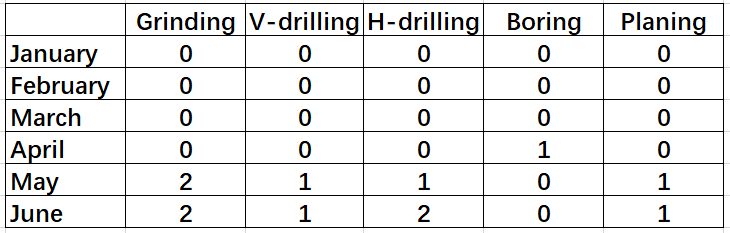
\includegraphics[width=12cm]{1.PNG}
      %	\caption{Example of inverting the color}
      %	\label{fig1}
     % \end{figure} 
 	   As we assume, the plane has been divided by k lines, and has been colored successfully. Then we add anothor line and name it $\lambda$, now we call the part at the right of $\lambda$ "$R$part", and the other one is "$L$part".
       
       Then, we invert the color of every cell in $R$part as the fig1 (the yellow line is $\lambda$). As you can see,  the new graph is still colored successfully.
      
   
       Now, we will prove its rationality. Because we only propose the $R$part, so every adjacent cells in $L$part stay the same and have different colors. Also, all of the cells in $R$part change their color, so every adjacent cells in $R$part still have different colors too.
       
       Then, about the ones next to the $\lambda$.They used to be unbroken, but are separated by the $\lambda$. Since we change the colors of the ones in $R$part, these changed cells have different colors with the left-adjacent ones.
       
       Now, every adjacent cells have different colors and  $P(k+1)$ is true. 
     
       
        
   \end{proof}

\end{enumerate}

\vspace{20pt}

\textbf{Remark:} You need to include your .pdf and .tex files in your uploaded .rar or .zip file.

%========================================================================
\end{document}
